\section{Formal: Parsing, Lexing, \& Grammar Types}
\subsection{Parsing Generators \& Grammar Types}


Lexical analysis and parsing are closely linked to 
compiler design. Though instead of writing such parsers by 
hand, we will use \textbf{parser generators}:

\begin{Def}[Parser Generators]

    \label{def:parser-generator}
    Parser generators are programs that take a representation of formal grammar as input and produces a parser as output.
\end{Def}

\noindent
We'll use \textbf{Menhir} for OCaml. There are other options but this suffices for our needs.
\begin{Def}[Menhir]

    Menhir is an LR(1) parser generator for OCaml. LR(1) stands for:
    \begin{itemize}
        \item \textbf{L}: Left-to-right scanning of the input.
        \item \textbf{R}: Rightmost derivation in reverse. Meaning, it builds the parse tree from the leaves up to the root.
        \item \textbf{(1)}: One symbol of lookahead. This means that the parser can look at one token ahead in the input stream to make parsing decisions.
    \end{itemize}
    \noindent
    Users input small OCaml snippets to define the production rules of the grammar.
\end{Def}

\newpage 

\noindent
A quick aside on Domain Specific Languages (DSLs):

\begin{Def}[Domain Specific Language (DSL)]

    A domain-specific language (DSL) is a programming language or specification language dedicated to a particular problem domain.
    An example of a DSL is SQL, as its only purpose is to query databases. This is in contrast to general-purpose languages like Python, which can be used for a wide range of applications.

\end{Def}

\noindent
Now we discuss \textbf{Extended BNF (EBNF)}, which allows us to be more expressive in our grammars with less noise.

\begin{Def}[Extended BNF (EBNF)]

\label{def:ebnf}
Extended Backus-Naur Form (EBNF) is a notation for specifying formal grammars, building upon BNF (Backus-Naur Form) by introducing syntactic extensions for greater clarity and brevity.
EBNF includes the following additional constructs:

\begin{itemize}
    
    \item \texttt{|} — alternation: denotes choice between patterns.
    \begin{itemize}
        \item \textbf{E.g.,}  \snippet{<letter> ::= A | B | C}, means that <letter> can be A, B, or C.
    \end{itemize}
    \item \texttt{\{\ldots \}} — repetition: the enclosed pattern may repeat \underline{\textbf{zero} or more times}.
    \begin{itemize}
        \item \textbf{E.g.,}  \snippet{<digits> ::= \{0 | 1 | 2 | 3 | 4 | 5 | 6 | 7 | 8 | 9\}}, matches:
        \begin{itemize}
            \item[>] \texttt{"0"}, \texttt{"320"}, \texttt{"11235813"}
        \end{itemize}
    \end{itemize}
    \item \texttt{[\ldots ]} — optionality: the enclosed pattern may appear zero or one time.
    \begin{itemize}
        \item \textbf{E.g.,} \snippet{<number> ::= ["-"] <digits>}, matches:
        \begin{itemize}
            \item[>] \texttt{"1"}, \texttt{"-320"}
        \end{itemize}
    \end{itemize}
    \item \texttt{(\ldots )} — grouping: used to group sequences or alternatives.
    \begin{itemize}
        \item \textbf{E.g.,} \snippet{<sum> ::= <number> {("+" | "-") <number>}}, matches:
        \item [>] \texttt{"1 + 2 - 3"}, \texttt{"-1 + 2"}, \texttt{"5"}
        \end{itemize}
    \item \texttt{"\ldots"} — terminal strings may be written in quotes. This clears ambiguity between terminal and non-terminal symbols.
    \begin{itemize}
        \item \textbf{E.g.,} in \snippet{<digit> ::= A | B | C}, it's clear that A, B, and C refer to non-terminal symbols. However, in the expression \snippet{<expr> ::= <expr> | "(" <expr> ")"}, the parenthesis are \textbf{crucial} in indicating that it is not grouping notation.
    \end{itemize}
\end{itemize}
\end{Def}

\newpage

\noindent
Let's elaborate more on \snippet{<digits>} from above:
\begin{Example}[Dealing with Optionality]

    In our previous grammar from Definition (\ref{def:ebnf}), we had:
    \begin{lstlisting}[numbers=none]
        <digit> ::= {0 | 1 | 2 | 3 | 4 | 5 | 6 | 7 | 8 | 9}
    \end{lstlisting}
    which matched:
    \begin{itemize}
        \item[>] \texttt{"0"}, \texttt{"320"}, \texttt{"11235813"}
    \end{itemize}

    \noindent
    But also unintentionally matched:
    \begin{itemize}
        \item[>] \texttt{""} \hfill \textit{(empty string)}
        \item[>] \texttt{"000"}, \texttt{"0123"} \hfill \textit{(leading zeros)}
    \end{itemize}
    
    \noindent
    Let's first fix the empty string case:
    \begin{lstlisting}[numbers=none]
        <digit> ::= 0 | 1 | 2 | 3 | 4 | 5 | 6 | 7 | 8 | 9
        <digits> ::= <digit> {<digit>}
    \end{lstlisting}

    \noindent
    To restrict leading zeros (e.g., for natural numbers), we refine further:
    \begin{lstlisting}[numbers=none]
        <nonzero> ::= 1 | 2 | 3 | 4 | 5 | 6 | 7 | 8 | 9
        <digits> ::= "0" | <nonzero> {<digit>}
    \end{lstlisting}

    \noindent
    Adding quotes around \snippet{0} is a stylistic choice and does not change the meaning of the grammar. We could have written:
    \begin{lstlisting}[numbers=none]
        <nonzero> ::= "1" | "2" | "3" | "4" | "5" | "6" | "7" | "8" | "9"
        <digits> ::= "0" | <nonzero> {<digit>}
    \end{lstlisting}
    \noindent
    Or without quotes, it doesn't matter as long as there is no ambiguity.
\end{Example}

\noindent
To be more precise with our language we briefly discuss \textbf{Automata Theory} and types of grammars:

\begin{Def}[Automata Theory]

    In mathematics, an automaton (Plural form: automata) is an abstract machine that follow a sequence of states (similar to a 
    flowchart). A finite number of states describe a \textbf{finite automaton (FA)} or \textbf{finite-state machine (FSM)}.
    \end{Def}

\begin{Tip}
    Automata comes from the Greek word $\alpha\upsilon\tau\acute{o}\mu\alpha\tau o\varsigma$ (autómatos), which means ``self-acting, self-willed, self-moving"
\end{Tip}

\newpage 


\noindent
Consider the following automaton described by a state machine diagram:

\begin{figure}[h]
    \centering
    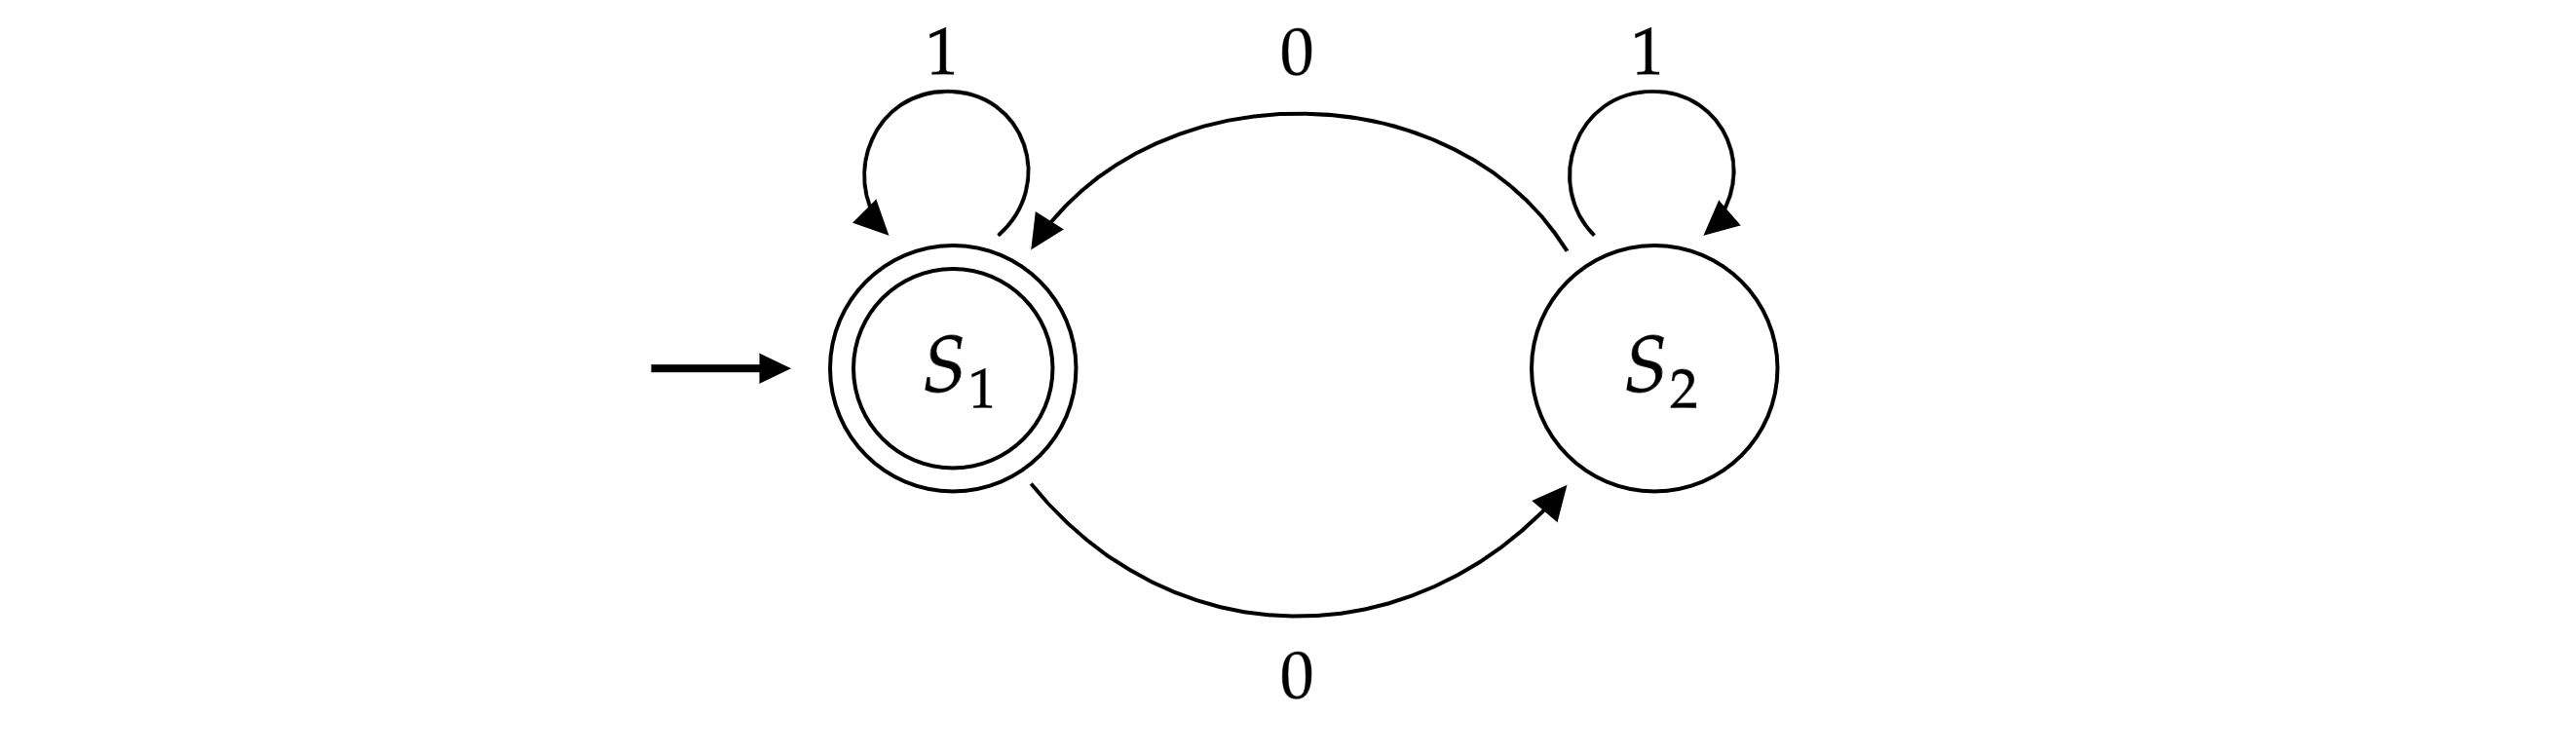
\includegraphics[width=\textwidth]{Sections/Parse/state.png}
    \caption{An automaton represented as a state-machine diagram. This state-machine generates binary strings with an even number of 0's.
    There are two states, $S_1$ and $S_2$. The automaton starts in state $S_1$ as shown by the arrow coming from blank space. The double
    circle indicates the \textbf{accepting state}, at which the automaton may terminate.}
    \label{fig:fa}
\end{figure}

\begin{Def}[Grammar Types]

    In formal language theory, grammars are classified into a hierarchy based on their generative power. This classification, known as the \textbf{Chomsky hierarchy}, comprises four primary types that utilize BNF:

    \begin{itemize}
        \item \textbf{Type 3: Regular Grammars} \\
        Generate \textbf{regular languages}, which can be recognized by finite automata. These grammars can describe simple flat patterns, but cannot handle nested or recursive structures.

        \item \textbf{Type 2: Context-Free Grammars (CFGs)} \\
        Generate \textbf{context-free languages} and are recognized by pushdown automata. A \textbf{pushdown automaton} is a finite automaton extended with a stack—a Last-In, First-Out (LIFO) memory structure. This allows it to handle nested and recursive structures, such as balanced parentheses.

        \item \textbf{Type 1: Context-Sensitive Grammars} \\
        Generate \textbf{context-sensitive languages} and are recognized by linear bounded automata. A \textbf{linear bounded automaton} is a Turing machine where the tape is limited to a length proportional to the input size. This constraint gives it more power than pushdown automata but less than unrestricted Turing machines.

        \item \textbf{Type 0: Unrestricted Grammars} \\
        Generate \textbf{recursively enumerable languages} and are recognized by Turing machines. These grammars have no restrictions on production rules and can describe any computable language, though some of these languages are undecidable.
    \end{itemize}
\end{Def}

\newpage 

\noindent
We can visualize the Chomsky hierarchy as follows:

\begin{figure}[h]
    \centering
    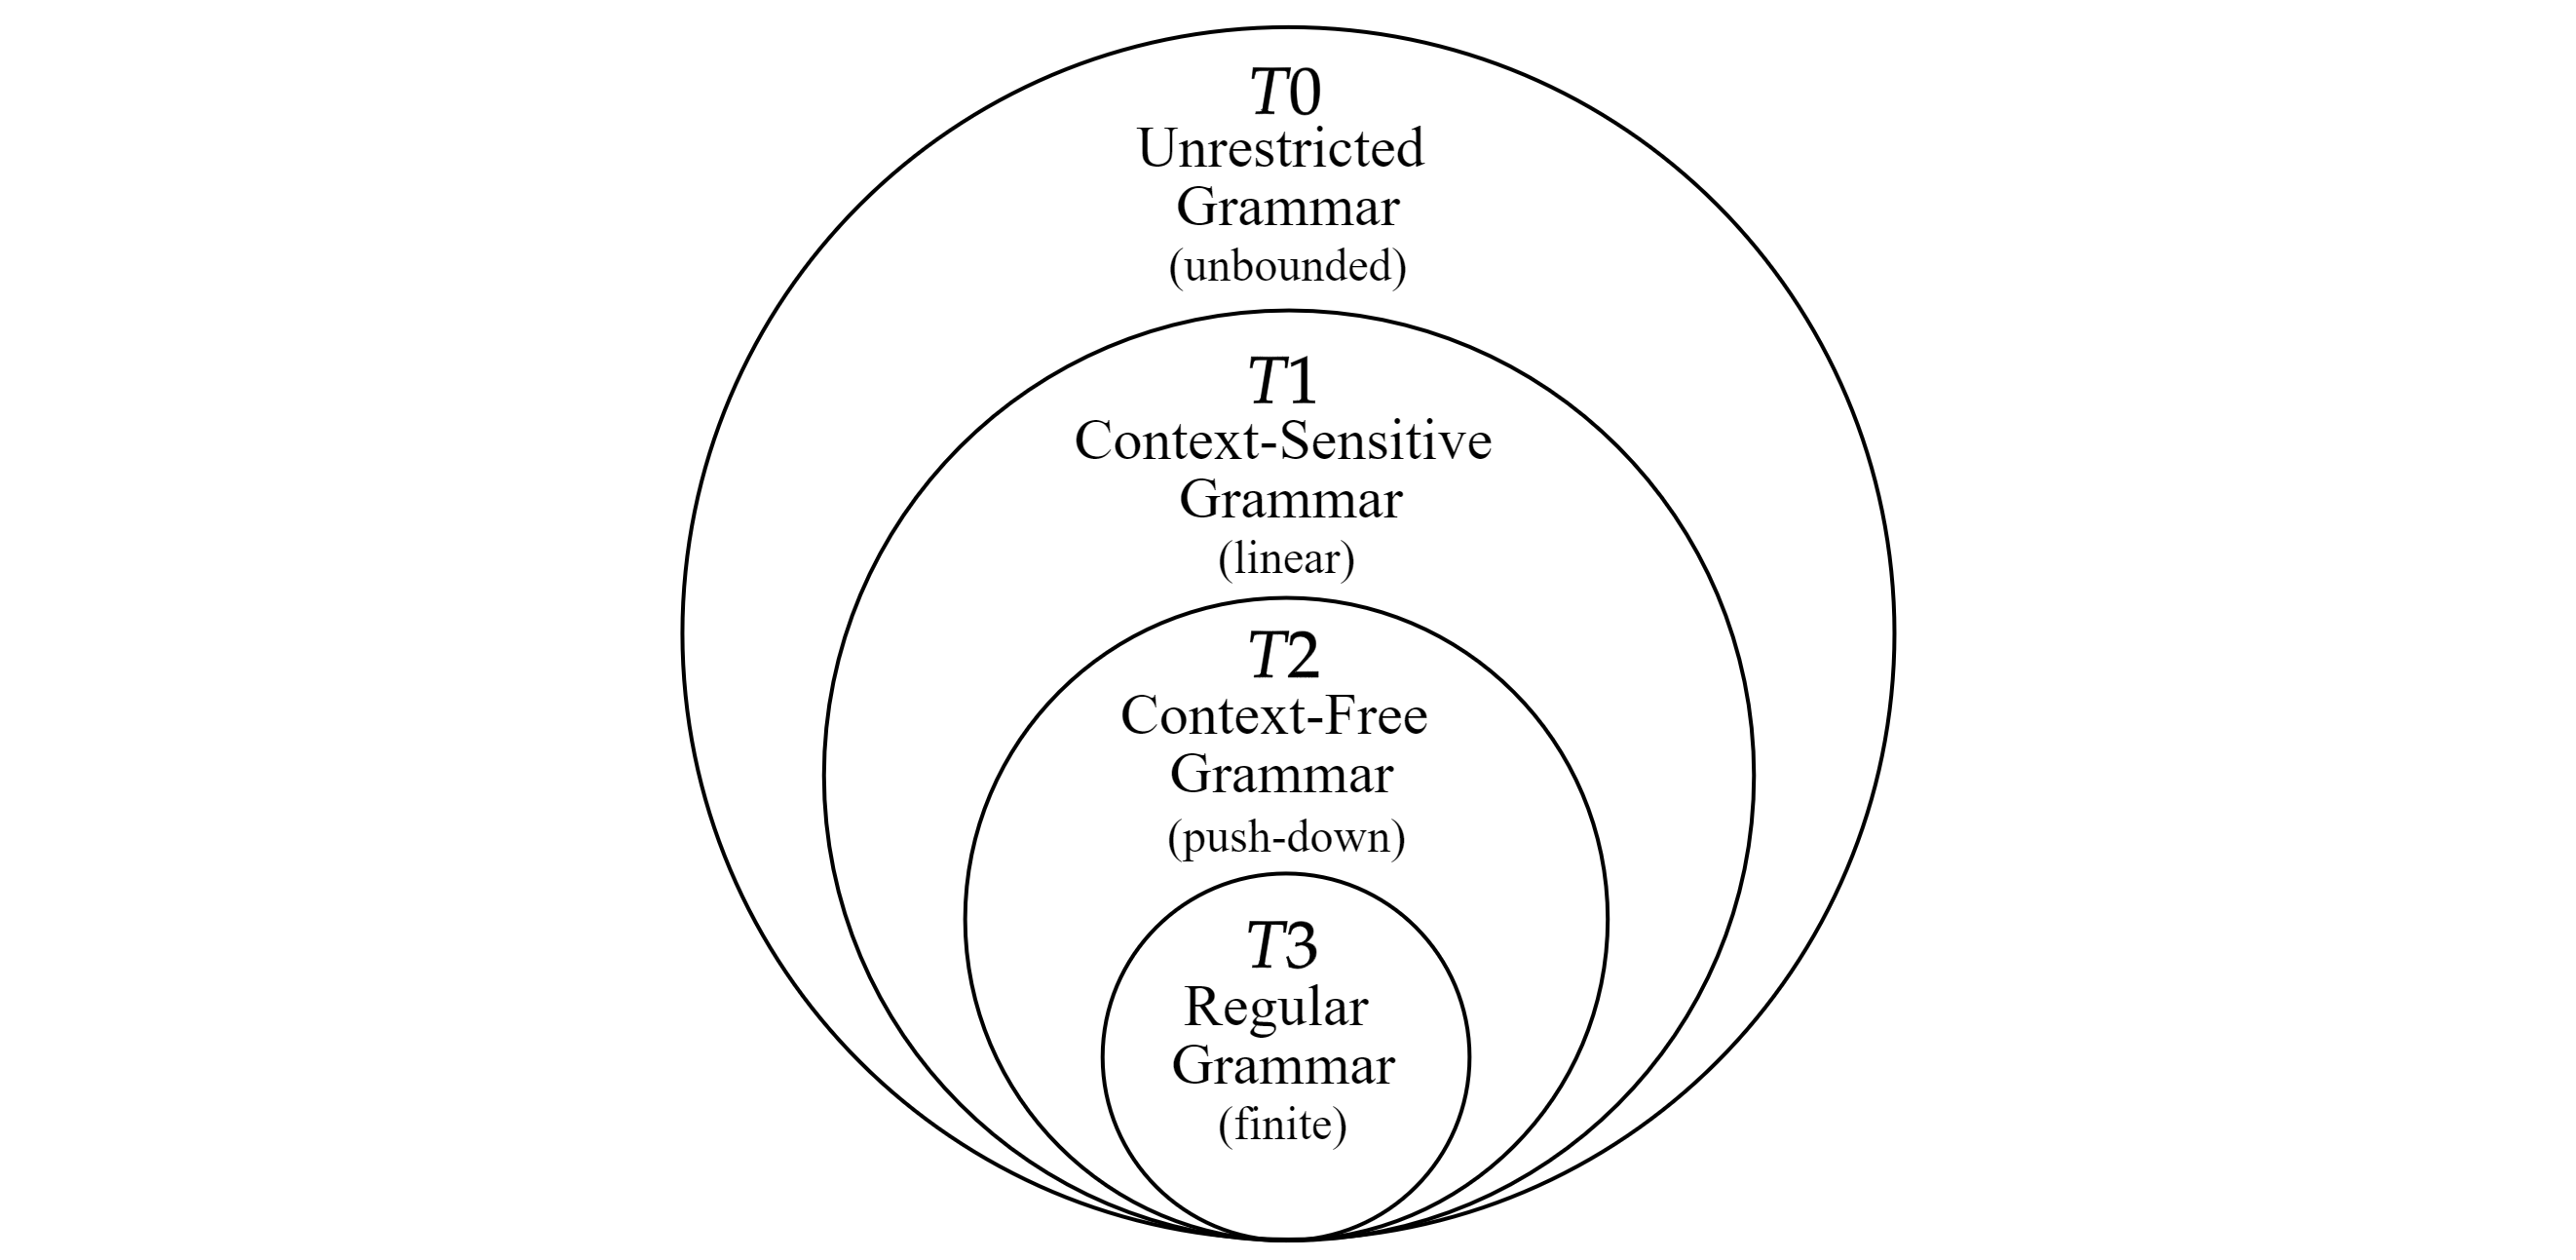
\includegraphics[width=\textwidth]{Sections/Parse/chom.png}
    \caption{
        The Chomsky hierarchy: 
        $T_3$ finite automata (regular expressions), 
        $T_2$ pushdown automata (context-free grammars),
        $T_1$ linear bounded automata (context-sensitive grammars),
        and $T_0$ Turing machines (unrestricted grammars).
    } 
    \label{fig:chomsky}
\end{figure}

\begin{Def}[Regular Expressions (Regex)]

    \label{def:regex}
    Regular expressions (Regex) provide a compact way to describe patterns in regular grammars:
    
    \begin{itemize}
        \item \texttt{a} — a single \textbf{terminal} symbol is itself a regex.
       
    
        \item \texttt{[t1 t2 \ldots tk]} — character class: matches any one of the listed characters.
        
    
        \item \texttt{(e1 | e2 | \ldots | ek)} — alternation: matches any one of the enclosed expressions.
       
    
        \item \texttt{exp*} — repetition: matches \underline{\textbf{zero or more occurrences}} of \texttt{exp}.
      
    
        \item \texttt{exp+} — repetition: matches \underline{\textbf{one or more occurrences}} of \texttt{exp}.
        
    
        \item \texttt{exp?} — optional: matches \underline{\textbf{zero or one occurrence}} of \texttt{exp}.
        
    \end{itemize}
    
    \noindent
    \textbf{E.g.,} the regex \texttt{(a|b)*c} matches any string of a's and b's followed by a c, such as:
    \begin{itemize}
        \item[>] \texttt{"abc"}, \texttt{"aabbbbc"}, \texttt{"c"}
    \end{itemize}
   
    \noindent
    This is just a small subset of the Regex syntax. To learn more, consider the following resource:
    \url{https://regexlearn.com/}
    \end{Def}
\newpage 
\subsection{Menhir: Simple Lexing \& Parsing }
\noindent
To formally retouch on the definitions of lexing:

\begin{Def}[Lexical Analysis]

    \label{def:lexical-analysis}
    Lexical analysis concerns itself with the \textbf{tokenization} of a program. In particular, converting a stream 
    of characters into a stream of tokens (whitespace and comments are ignored).

    Lexing (to lex) works by scanning the input for the next longest valid token. Then 
    it returns that token and the remaining input to lex.\\

    \noindent
    \textbf{E.g.,} \snippet{" let@\#\_)(\$\#@\_J\_@O\#GKJ"} gives us \snippet{(LET, "@\#\_)(\$\#@\_J\_@O\#GKJ")}, where 
    \snippet{LET} is the token and \snippet{"@\#\_)(\$\#@\_J\_@O\#GKJ"} is the remaining input, which is most likely to result in an error 
    (unless the lexer is designed to handle such cases).
\end{Def}

\noindent
We will now create a lexer and parser for a simple toy-language that only has 
addition, subtraction, multiplication, and division.
Menhir should already be installed from the onboarding Section (\ref{subsec:opam_packages}).



\begin{Example}[Simple Lexer \& Parser (Part 1)]

    \label{ex:lexer-parser}
    Let's create a simple lexer and parser for a toy language that only has addition, subtraction, multiplication, and division.
    We will use Menhir to generate the parser.\\

    \noindent
    Let's create the project: 
    \begin{lstlisting}[numbers=none]
        dune init proj small_arith
        cd small_arith
    \end{lstlisting}

    \noindent
    This should create: \\

    \noindent
    \rule{\textwidth}{0.4pt} 
    \dirtree{%
    .1 small\_arith/.
    .2 \_build/.
    .3 log.
    .2 bin/.
    .3 dune.
    .3 main.ml.
    .2 dune-project.
    .2 lib/.
    .3 dune.
    .2 small\_arith.opam.
    .2 test/.
    .3 dune.
    .3 test\_small\_arith.ml.
    }
    \noindent
    \rule{\textwidth}{0.4pt} \\
\end{Example}


\newpage 

\begin{Example}[Simple Lexer \& Parser (Part 2)]

    \noindent
    Create these new files, \snippet{lib/ast.ml}, \snippet{lib/lexer.mll}, and \snippet{lib/parser.mly}:
    \begin{lstlisting}
        touch lib/dune lib/ast.ml lib/lexer.mll lib/parser.mly
    \end{lstlisting}

\begin{itemize}
    \item \snippet{ast.ml} — A regular OCaml source file (\texttt{.ml}) where we define the core data structures via ADTs, which will generate the \textbf{abstract syntax tree (AST)} for our language.

    \item \snippet{lexer.mll} — The (\texttt{.mll}) extension to signal it will be processed by \textbf{OCamllex}, a lexer generator. Here, we write rules using regular-expression-like syntax to convert raw strings into \textbf{tokens} like \texttt{NUM}, \texttt{ADD}, and \texttt{LPAREN}.

    \item \snippet{parser.mly} — The (\texttt{.mly}) extension is handled by \textbf{Menhir}. It defines the \textbf{grammar} of our language. The result of parsing is an AST defined in \snippet{ast.ml}.
\end{itemize}

\noindent
\textbf{Together:} 
\texttt{Input String} $\rightarrow$ \texttt{Lexer (mll)} $\rightarrow$ \texttt{Tokens} $\rightarrow$ \texttt{Parser (mly)} $\rightarrow$ \texttt{AST (ml)}

\noindent
\rule{\textwidth}{0.4pt}\\

\noindent
Lets begin by defining the AST in \snippet{ast.ml}:
\begin{lstlisting}[numbers=none]
    (* ast.ml *)
    type bop = Add | Sub | Mul | Div 
    
    type expr =
      | Var of string
      | Num of int
      | Let of string * expr * expr
      | Bop of bop * expr * expr
    
    type prog = expr
    \end{lstlisting}

\noindent
    The above code defines the abstract syntax tree (AST) for our toy language. It includes:
    \begin{itemize}
        \item \texttt{bop} — a type for binary operators (addition, subtraction, multiplication, division).
        \item \texttt{expr} — a type for expressions, which can be a variable, number, let-binding, or binary operation.
        \item \texttt{prog} — a type for the program, which is just an expression.
    \end{itemize}

    \noindent
    This should be familiar from the BNF grammar we've discussing.
\end{Example}

\newpage 


\begin{Example}[Simple Lexer \& Parser (Part 4)]

    Now let's define our lexer in \snippet{lib/lexer.mll}:
    
    \begin{lstlisting}[numbers=none]
    (* lexer.mll *)
    {
        open Parser
    }

    (* Regex for tokens *)
    let whitespace = [' ' '\t' '\n' '\r']+
    let var = ['a'-'z' '_'] ['a'-'z' 'A'-'Z' '0'-'9' '_' '\'']*
    let num = ['0'-'9']+

    rule read = parse
        | whitespace { read lexbuf }
        | "let"      { LET }
        | "in"       { IN }
        | "="        { EQ }
        | "+"        { ADD }
        | "-"        { SUB }
        | "*"        { MUL }
        | "/"        { DIV }
        | "("        { LPAREN }
        | ")"        { RPAREN }
        | num        { NUM (int_of_string (Lexing.lexeme lexbuf)) }
        | var        { VAR (Lexing.lexeme lexbuf) }
        | eof        { EOF }
    \end{lstlisting}
    
    \begin{itemize}
        \item \snippet{lexbuf}: short for \textbf{``lexing buffer,''} is an object created by the OCaml stdlib. It stores the input string and tracks the position of the lexer as it reads through.
        
        \item \snippet{read lexbuf}: A recursive call to the lexer function. It's used to \textbf{skip over whitespace}. When the lexer sees a space or newline, it just calls itself again to scan the next part of the input.
    
        \item \snippet{Lexing.lexeme lexbuf}: This function returns the \textbf{exact substring} that was matched by our Regex.
         For example, if the input is \texttt{"42 + 1"} and we match \snippet{num}, then\\
        \snippet{Lexing.lexeme lexbuf} returns \texttt{"42"} as a string. We then convert it to an integer.

        \item \snippet{rule read = parse}: This defines the main lexer function. The \snippet{read} is the entry point of the lexer. The \snippet{parse} keyword indicates parsing rules for the input to match against.
    \end{itemize}
    
    
\end{Example}
        
\newpage 

\begin{Example}[Simple Lexer \& Parser (Part 5)]

    Finally the parser in \snippet{lib/parser.mly} utilizing our \snippet{ast.ml} (Moreover on the next page.):
    
    \begin{lstlisting}[numbers=none]
    %{
      open Ast
    %}
    
    %token LET EQ IN
    %token ADD SUB MUL DIV
    %token LPAREN RPAREN
    %token <int> NUM
    %token <string> VAR
    %token EOF
    
    %left ADD SUB
    %left MUL DIV
    
    %start <Ast.prog> prog
    %%
    
    prog:
      | e = expr; EOF { e }
    
    expr:
      | LET; x = var; EQ; e1 = expr; IN; e2 = expr
        { Let (x, e1, e2) }
      | e = expr1 { e }
    
    %inline bop:
      | ADD { Add }
      | SUB { Sub }
      | MUL { Mul }
      | DIV { Div }
    
    expr1:
      | e1 = expr1; op = bop; e2 = expr1
        { Bop (op, e1, e2) }
      | n = num { Num n }
      | v = var { Var v }
      | LPAREN; e = expr; RPAREN { e }
    
    num:
      | n = NUM { n }
    
    var:
      | x = VAR { x }
    \end{lstlisting}

    \noindent
    
    \end{Example}
    

    \begin{Example}[Simple Lexer \& Parser (Part 5a)]

        The \snippet{parser.mly} file looks quite different from regular OCaml code because it follows the syntax of Menhir (an LR(1) parser generator). Let's walk through its structure:
        
        \begin{itemize}
            \item \snippet{\%\{ ... \%\}} — Opens a block of OCaml code. We use it to import our AST module.
        
            \item \snippet{\%token} — Declares the tokens the parser will receive from the lexer. If tokens carry data integer or string, we write it as:
            \begin{lstlisting}[numbers=none]
        %token <int> NUM
        %token <string> VAR
            \end{lstlisting}
        
            \item \snippet{\%left} — Defines left-associativity, and precedence is by order of declaration:
            \begin{lstlisting}[numbers=none]
        %left ADD SUB
        %left MUL DIV
            \end{lstlisting}
            means that \snippet{MUL} and \snippet{DIV} bind more tightly than \snippet{ADD} and \snippet{SUB}. All are left-associative. This prevents ambiguity in expressions like \texttt{3 + 4 * 2}.
        
            \item \snippet{\%start <Ast.prog> prog} — The entry point of the parser is the rule \snippet{prog}. The return type is \snippet{Ast.prog} from our AST module.
           
        
            \item \snippet{<name>:} — Each rule has the form:
            \begin{lstlisting}[numbers=none]
        name:
          | pattern1 { action1 }
          | pattern2 { action2 }
            \end{lstlisting}
            Think of it as EBNF, but instead we use OCaml pattern matching syntax.
        
            \item \snippet{\%inline <name>:} — A helper rule that lets us \textbf{macro} grammar patterns into a single variable without generating a new nonterminal or type (cannot be recursive):
            \begin{lstlisting}[numbers=none]
        %inline bop:
          | ADD { Add }
          | SUB { Sub }
          | ...
            \end{lstlisting}
        
        \end{itemize}
        \end{Example}

        \newpage 

\begin{Example}[Simple Lexer \& Parser (Part 5b)]

    Let's look closely at the following grammar rule:
    
    \begin{lstlisting}[numbers=none]
    expr:
        | LET; x = var; EQ; e1 = expr; IN; e2 = expr
        { Let (x, e1, e2) }
    \end{lstlisting}
    
    \begin{itemize}
        \item Each item before the `\texttt{\{}' is a \textbf{token} (e.g., \snippet{LET}, \snippet{EQ}, \snippet{IN}) or a \textbf{nonterminal rule} (e.g., \snippet{var}, \snippet{expr}).
        \item When a nonterminal is matched, we can bind its result using \snippet{name = rule}. For example, \snippet{x = var} means: “run the \snippet{var} rule and bind its result to \snippet{x}.”
        \item The block in \texttt{\{ \}} is an OCaml expression that builds an AST node using the bound variables.
        Notice, \snippet{Let (x, e1, e2)} our ADT constructor from \snippet{ast.ml}.
    \end{itemize}
    
    \noindent
    \rule{\textwidth}{0.4pt}\\

    \noindent
    When we parse a string like:
    
    \begin{lstlisting}[numbers=none]
    let x = 3 + 4 in x * 2
    \end{lstlisting}
    
    \noindent
    The lexer produces a stream of tokens:
    
    \begin{lstlisting}[numbers=none]
 [LET; VAR("x"); EQ; NUM(3); ADD; NUM(4); IN; VAR("x"); MUL; NUM(2); EOF]
    \end{lstlisting}
    
    \noindent
    Then, the parser:
    \begin{itemize}
        \item Sees \snippet{LET}, then \snippet{VAR("x")} → runs the \snippet{var} rule, binds to \snippet{x}.
        \item Sees \snippet{EQ}, then parses the expression \snippet{3 + 4} using the \snippet{expr} rule, binds to \snippet{e1}.
        \item Sees \snippet{IN}, then parses the expression \snippet{x * 2}, binds to \snippet{e2}.
    \end{itemize}
    
    \noindent
    Finally, it constructs:
    
    \begin{lstlisting}[numbers=none]
    Let (x, e1, e2)
    \end{lstlisting}
    
    \noindent
    This is now a fully constructed OCaml value using the constructors we defined in \snippet{ast.ml}.
    
    \end{Example}
            
    \newpage 

\begin{Example}[Simple Lexer \& Parser (Part 6)]

    Now that we've written our AST, lexer, and parser, we need to set up Dune so we can compile everything and test it in \texttt{utop}.\\
    
    \noindent
    First, open your \snippet{dune-project} file and add the following line at the bottom to enable Menhir:
    
    \begin{lstlisting}[numbers=none]
    (using menhir 3.0)
    \end{lstlisting}
    
    \noindent
    Your complete \snippet{dune-project} should now look like:
    
    \begin{lstlisting}[numbers=none]
    (lang dune 3.0)
    (name small_arith)
    (using menhir 3.0)
    \end{lstlisting}
    
    \noindent
    Next, open \snippet{lib/dune}:
    
    \begin{lstlisting}[numbers=none]
    (library
        (name small_arith))
    
    (ocamllex lexer)
    (menhir (modules parser))
    \end{lstlisting}
    
    \noindent
    Create a \snippet{lib/demo.ml} file to test the lexer and parser:
    \begin{lstlisting}[numbers=none]
    let parse s =
        try Some (Parser.prog Lexer.read (Lexing.from_string s))
        with _ -> None
    \end{lstlisting}
    
    \noindent
    From the root of your project, run:
    
    \begin{lstlisting}[numbers=none]
    dune build
    dune utop lib
    \end{lstlisting}
    
    \noindent
    In \texttt{utop}, you can test the parser like this:
    
    \begin{lstlisting}[numbers=none]
    # open Demo;;
    # parse "let x = 3 + 4 in x * 2";;
    - : prog option =
    Some
    (Let ("x",
         Bop (Add, Num 3, Num 4),
         Bop (Mul, Var "x", Num 2)
    ))
    \end{lstlisting}
    \end{Example}
        
        
